\documentclass[11pt,a4paper]{article}

\usepackage[margin=2.5cm]{geometry}
\usepackage{booktabs}
\usepackage{float}
\usepackage{tabularx}
\usepackage{xltabular}
\usepackage{array}
\usepackage{enumitem}
\usepackage{totcount}
\usepackage{fancyhdr}
\usepackage{lastpage}
\usepackage{tikz}
\usetikzlibrary{arrows.meta,positioning,calc}
\usepackage[hidelinks]{hyperref}
\setlength{\emergencystretch}{1.5em}

% Section numbers in the same style as the ConOps: 1.0, 1.1.
\renewcommand{\thesection}{\arabic{section}.0}
\renewcommand{\thesubsection}{\arabic{section}.\arabic{subsection}}

% Controlled-document header on every page.
\newcommand{\docref}{Reference TBD}
\newcommand{\docrev}{Issue 1, Rev.~0 --- DRAFT}
\pagestyle{fancy}
\fancyhf{}
\lhead{\footnotesize Fail-Safe In-Orbit Reprogramming of a Spacecraft Controller --- Hardware Trade Study}
\lfoot{\small \docref}
\cfoot{\small \docrev}
\rfoot{\small Page \thepage\ of \pageref{LastPage}}

% Open items. TBD = not known. TBR = proposal awaiting the author's
% acceptance. Listed in App. B; totals counted, not typed.
\newtotcounter{tbd}
\newtotcounter{tbr}
\newcommand{\tbditem}[2]{\refstepcounter{tbd}\label{tbd:#1}\item[TBD-\thetbd] #2}
\newcommand{\tbritem}[2]{\refstepcounter{tbr}\label{tbr:#1}\item[TBR-\thetbr] #2}
\newcommand{\tbd}[1]{\mbox{\textbf{[\hyperref[tbd:#1]{TBD-\ref*{tbd:#1}}]}}}
\newcommand{\tbr}[1]{\mbox{\textbf{[\hyperref[tbr:#1]{TBR-\ref*{tbr:#1}}]}}}

% Keeps words whole inside figure boxes.
\newcommand{\nohyph}{\hyphenpenalty=10000\exhyphenpenalty=10000\relax}

\setlist[description]{style=multiline,leftmargin=2.2cm,nosep,font=\normalfont\bfseries}
\setlist[itemize]{nosep}

\begin{document}

\thispagestyle{fancy}
\begin{center}
{\LARGE\bfseries Fail-Safe In-Orbit Reprogramming\\[0.2em] of a Spacecraft Controller\par}
\vspace{0.4em}
{\Large Hardware Trade Study\par}
\vspace{1em}
\begin{tabular}{@{}ll@{}}
Reference & TBD \tbd{ref} \\
Issue / revision & Issue 1, Revision 0 --- DRAFT \\
Date & 12 October 2026 \\
Author & Andrew Toma \\
Open items & \total{tbd} TBD, \total{tbr} TBR (App.~B) \\
\end{tabular}
\end{center}

\subsection*{Document change record}
\begin{tabular}{@{}llll@{}}
\toprule
Issue & Rev. & Date & Change \\
\midrule
1 & 0 & 2026-10-12 & First draft \\
\bottomrule
\end{tabular}

% ===========================================================================
\section{Purpose and Scope}
This study chooses the hardware of the bench on which the System is built and
verified. It measures each candidate against the hardware needs of the
architecture [2,~Sec.~8.0] and the bench needs of the verification plan
[3,~Sec.~5.0], and prefers hardware the author already owns. It chooses in two
steps: a first bench of owned boards only, and the parts the full bench adds.

% ===========================================================================
\section{Documents}
\noindent [1] NASA, \emph{NASA Systems Engineering Handbook},
NASA/SP-2016-6105 Rev~2, 2016.

\noindent [2] \emph{Fail-Safe In-Orbit Reprogramming of a Spacecraft
Controller --- Software Architecture}, Issue~1, Revision~0, Draft.

\noindent [3] \emph{Fail-Safe In-Orbit Reprogramming of a Spacecraft
Controller --- Verification Plan}, Issue~1, Revision~0, Draft.

\noindent [4] STMicroelectronics, \emph{STM32G431xB Datasheet}, DS12589 Rev~6.

\noindent [5] STMicroelectronics, \emph{STM32G4 Series Reference Manual},
RM0440 Rev~9.

\noindent [6] STMicroelectronics, \emph{STM32G4 Nucleo-32 Board (MB1430)},
UM2397 Rev~2.

\noindent [7] STMicroelectronics, \emph{Introduction to System Memory Boot
Mode on STM32 MCUs}, AN2606 Rev~70.

\noindent [8] STMicroelectronics, \emph{Discovery Kit with STM32MP257F MPU},
UM3385 Rev~2.

\noindent [9] Texas Instruments, \emph{THVD14xx 3.3-V to 5-V RS-485
Transceivers}, SLLSEY3E, 2019.

\noindent [10] Texas Instruments, \emph{TCAN33x 3.3V CAN Transceivers with CAN
FD}, SLLSEQ7F, 2025.

\noindent [11] Texas Instruments, \emph{TMUX1574 2:1 (SPDT) 4-Channel Switch},
SCDS391C, 2019.

\noindent [12] Linux kernel, \texttt{drivers/net/can/usb/gs\_usb.c}, mainline,
read 12 October 2026.

\noindent [13] \texttt{uhubctl} project, \emph{README}, read 12 October 2026.

\noindent [14] STMicroelectronics, \emph{STM32G474xB/xC/xE Datasheet}, DS12288
Rev~3 (distributor copy; later revisions not obtained).

\noindent [15] STMicroelectronics, \emph{STM32G491xC/xE Datasheet}, DS13122
Rev~4 (distributor copy).

\noindent [16] STMicroelectronics, \emph{STM32G4 Nucleo-64 Boards (MB1367)},
UM2505 Rev~4 (distributor copy; Rev~7 not obtained).

\noindent [17] D.~Owens et al., ``Efficient and Side-Channel Resistant Ed25519
on ARM Cortex-M4'', \emph{IEEE Trans.\ Circuits and Systems~I}, vol.~71,
no.~6, June 2024.

\noindent [18] Linux kernel, \texttt{Documentation/networking/can.rst},
mainline, read 12 October 2026.

% ===========================================================================
\section{Criteria}
Each need of the architecture and of the verification plan is a criterion.
Each candidate gets one of four answers for each criterion. Among candidates
that meet the needs, owned hardware comes first, then the lowest cost.

\smallskip
\noindent{\small\textbf{Legend.} MET: met as the board is. PARTLY: met only
with a board change, or with a limit stated beside it. NOT MET: not met.
TO MEASURE: settled only by a measurement on the bench [3,~Sec.~7.6].}

% ===========================================================================
\section{Controller}
Three boards are assessed: the NUCLEO-G431KB, which the author owns, and two
Nucleo-64 boards built on the same board design, the NUCLEO-G474RE and the
NUCLEO-G491RE [16,~p.~1]. A published Ed25519 verification on a Cortex-M4
takes 720\,000 cycles [17,~p.~2674]; two take about 8.5\,ms at 170\,MHz, a
figure measured on the bench for each board [3,~Sec.~7.6].

\smallskip
{\footnotesize\noindent\begin{tabularx}{\textwidth}{@{}>{\raggedright\arraybackslash}p{2.8cm}>{\raggedright\arraybackslash}X>{\raggedright\arraybackslash}X>{\raggedright\arraybackslash}X@{}}
\toprule
Need [2,~Sec.~8.0] & NUCLEO-G431KB & NUCLEO-G474RE & NUCLEO-G491RE \\
\midrule
Clock and RAM for two signature checks & TO MEASURE: 170\,MHz, 32\,KB SRAM [4,~pp.~1, 14] & TO MEASURE: 170\,MHz, 128\,KB SRAM [14,~Sec.~3.5, p.~20] & TO MEASURE: 170\,MHz, 112\,KB SRAM [15,~Sec.~3.5, pp.~18--19] \\
Flash; writing while running & PARTLY: 128\,KB, one bank; a page erase stalls code for up to 24.47\,ms [5,~p.~195; 4,~p.~107] & MET: 512\,KB in two banks, read-while-write with the DBANK option bit set [14,~Sec.~3.4, p.~19; 5,~Sec.~3.3.8, p.~108] & PARTLY: 512\,KB, one bank; erase stalls code [5,~p.~156] \\
UART for data link A & PARTLY: USART2 wired to the ST-LINK by default [6,~p.~16] & MET: UART5, apart from the factory loader's UARTs [14,~p.~75] & MET: UART5 [15,~Table~13, p.~65] \\
CAN FD controller & MET: one [4,~Table~13, p.~61] & MET: three [14,~Table~2, p.~15] & MET: two [15,~p.~14] \\
SWD with full memory access & PARTLY: reaches only the on-board ST-LINK [6,~pp.~22--23] & MET: PA13/PA14 on header CN7 pins 13 and 15 [16,~Table~16, p.~31] & MET: same board as the G474RE [16,~Table~16, p.~31] \\
Factory loader on its own UART & MET: USART1 [7,~Table~115, p.~274] & MET: USART1 to 3 [7,~Table~117, p.~279] & MET: USART1 to 3 [7,~Table~119, p.~285] \\
NRST and BOOT pins accessible & PARTLY: BOOT0 not on a header [6,~p.~16] & PARTLY: NRST on CN7 pin 14; BOOT0 on CN7 pin 7 but not connected by default [16,~Table~16, pp.~31--32] \tbd{boot0} & PARTLY: same board as the G474RE \\
Independent watchdog & MET [5,~p.~1557] & MET [5,~p.~1557] & MET [5,~p.~1557] \\
RTC with an independent clock source & PARTLY: internal oscillator only, 29.5 to 34\,kHz [4,~pp.~51, 105] & MET: 32.768\,kHz crystal fitted [16,~Sec.~6.5.2, p.~22] & MET: same board as the G474RE \\
Owned & YES & NO & NO \\
\bottomrule
\end{tabularx}}

% ===========================================================================
\section{Onboard Computer}
The only candidate is the STM32MP257F-DK, which the author owns. Its 40-pin
header carries one UART, USART6, on pins 8 and 10 [8,~Table~24, p.~35]. It
has two USB Type-A host ports [8,~p.~2].

\smallskip
{\small\noindent\begin{tabularx}{\textwidth}{@{}>{\raggedright\arraybackslash}p{4.2cm}l>{\raggedright\arraybackslash}X@{}}
\toprule
Need [2,~Sec.~8.0] & Answer & STM32MP257F-DK \\
\midrule
UART for data link A & MET & USART6 on the header [8,~Table~24, p.~35] \\
UART to the factory loader & PARTLY & No second UART documented on the header; a USB-to-RS-422 adapter on a host port meets it \tbd{uart2} \\
CAN FD controller with transceiver & PARTLY & No CAN signal on the header and no transceiver on the board [8,~Table~24, p.~35]; a USB CAN FD adapter meets it, with CAN FD support in the mainline Linux driver [12,~ll.~181, 969] \\
Four GPIOs: SWDIO, SWCLK, NRST, BOOT & MET & Free header pins, for example PZ0, PZ1 and PZ9 on pins 15, 16 and 13 [8,~Table~24, p.~35] \\
Storage for two firmware stores & MET & 8\,GB eMMC and a microSD slot [8,~pp.~2, 18] \\
\bottomrule
\end{tabularx}}

% ===========================================================================
\section{Interface Parts and Bench Tools}
No ready-made modules were found for the transceivers below; they are mounted
on small adapter boards.

\smallskip
{\small\noindent\begin{tabularx}{\textwidth}{@{}>{\raggedright\arraybackslash}p{3.6cm}>{\raggedright\arraybackslash}p{2.6cm}c>{\raggedright\arraybackslash}X@{}}
\toprule
Need & Candidate & Count & Facts \\
\midrule
RS-422 line drivers, data link A and factory loader & TI THVD1451 & 4 & 3 to 5.5\,V supply; full duplex; up to 50\,Mbps [9,~p.~1; Table~5, p.~4] \\
CAN FD transceiver & TI TCAN332G & 2 & Single 3.3\,V supply; CAN FD up to 5\,Mbps [10,~p.~1] \\
Debug port shared by the probe and the onboard computer [3,~Sec.~5.0] & TI TMUX1574 & 1 & Four 2:1 switches, so SWDIO, SWCLK, NRST and BOOT change over together; 1.5 to 5.5\,V supply [11,~p.~1] \\
Controller power cut at a chosen moment [3,~Sec.~5.0] & USB hub with per-port power switching & 1 & Switched from a script by \texttt{uhubctl} [13,~Sec.~What is USB per-port power switching?]; the hub model \tbd{hub} \\
Events time-stamped from one clock [3,~Sec.~5.0] & Logic analyzer & 1 & Model \tbd{analyzer} \\
Data link cut and bytes changed on command [3,~Sec.~5.0] & Board in the middle of the link & 1 & Board \tbd{linktool} \\
\bottomrule
\end{tabularx}}

% ===========================================================================
\section{Selection}

\subsection{First Bench}
The first bench uses only the two owned boards (Figure~\ref{fig:bench1}). The
NUCLEO-G431KB's USB plugs into a host port of the STM32MP257F-DK. Through the
on-board ST-LINK, one cable gives the onboard computer the controller's USART2
as data link A [6,~p.~16] and the controller's SWD port for the restore. Power
is cut by hand, and events are time-stamped by the onboard computer's clock.
It costs nothing.

\begin{figure}[H]
\centering
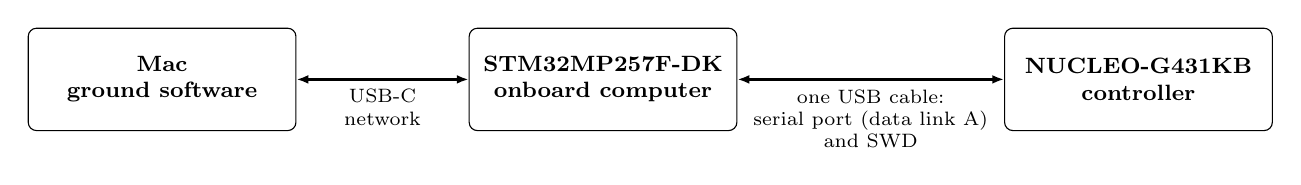
\begin{tikzpicture}[font=\scriptsize,
  unit/.style={draw, rounded corners=3pt, minimum width=3.4cm, minimum height=1.3cm, align=center, font=\footnotesize\bfseries},
  ar/.style={{Latex[length=1.5mm]}-{Latex[length=1.5mm]}, thick}]
\node[unit] (g) at (-0.6,0) {Mac\\ground software};
\node[unit] (o) at (5.0,0) {STM32MP257F-DK\\onboard computer};
\node[unit] (c) at (11.8,0) {NUCLEO-G431KB\\controller};
\draw[ar] (g) -- node[below, align=center]{USB-C\\network} (o);
\draw[ar] (o) -- node[below, align=center]{one USB cable:\\serial port (data link A)\\and SWD} (c);
\end{tikzpicture}
\caption{The first bench: owned hardware only.}
\label{fig:bench1}
\end{figure}

\noindent It shows the update, the trial, the return to the previous copy, the
refusal of damaged and forged images, and the restore of an erased controller.
It does not show data link B, the RS-422 and CAN electrical links, the restore
through the factory loader, SWD driven from the onboard computer's own pins, or
power cuts made by a script.

\subsection{Owned-Hardware Bench}
The bench then grows with jumper wires and one soldered wire, buying nothing
(Table~\ref{tab:wires}) \tbr{owned}. The onboard computer's second UART stands
in for data link B and also reaches the factory loader. Its NRST line resets
the controller at a chosen moment, in place of a power cut. A bench-only
program on the onboard computer drops, cuts or changes bytes on a link, in
place of a link tool. The CAN FD software is tested on each end alone: the
controller's with its CAN controller in loop-back test mode [5,~Sec.~44.2,
p.~1953], the onboard computer's on a virtual CAN interface, which sends and
receives CAN frames ``without real CAN controller hardware''
[18,~Sec.~The Virtual CAN Driver (vcan)]. Before wiring, the high level of a
header pin of the onboard computer is measured \tbd{level}.

\begin{table}[H]
\centering
{\small\begin{tabularx}{\textwidth}{@{}>{\raggedright\arraybackslash}p{3.4cm}>{\raggedright\arraybackslash}p{3.6cm}>{\raggedright\arraybackslash}X@{}}
\toprule
STM32MP257F-DK & NUCLEO-G431KB & Use \\
\midrule
USB Type-A port & USB port & Data link A (ST-LINK serial port); SWD for the restore and the debug probe \\
USART6 TX, CN5 pin 8 & PA10, CN4 pin 2 & Data link B and the factory loader's UART \\
USART6 RX, CN5 pin 10 & PA9, CN4 pin 1 & Data link B and the factory loader's UART \\
GND, CN5 pin 6 & GND, CN3 pin 2 & Common ground \\
PZ0, CN5 pin 15 & NRST, CN3 pin 3 & Reset, pulled low only \\
PZ1, CN5 pin 16 & PB8 (BOOT0), soldered wire & Boot pin for the factory loader \\
PZ9, CN5 pin 13 & PB0, CN4 pin 6 & Event line, time-stamped by the onboard computer \\
\bottomrule
\end{tabularx}}
\caption{Wiring of the owned-hardware bench [8,~Table~24, p.~35; 6,~Table~11, p.~22; 6,~p.~16].}
\label{tab:wires}
\end{table}

\noindent It runs every verification activity except those on the RS-422 and
CAN electrical links, on a true power cut, and on SWD driven from the onboard
computer's own pins. The parts of Section~6.0 add those later.

% ===========================================================================
\appendix
\renewcommand{\thesection}{\Alph{section}}

\section{Acronyms}
\begin{description}
\item[CAN FD] Controller Area Network with Flexible Data rate
\item[GPIO] General-purpose input/output
\item[NRST] Reset pin
\item[RTC] Real-time clock
\item[SWD] Serial Wire Debug
\item[TBD] To Be Determined
\item[TBR] To Be Resolved
\item[UART] Universal asynchronous receiver-transmitter
\item[USB] Universal Serial Bus
\end{description}

\section{Open Items}
The values below are not yet known.
\begin{description}
\tbditem{ref}{Project name and document reference.}
\tbditem{boot0}{The board change that connects BOOT0 to header CN7 on the
  Nucleo-64 boards; settled by the board schematic.}
\tbditem{uart2}{Whether the STM32MP257's pins can put a second UART and CAN FD
  on the header; settled by its datasheet.}
\tbditem{hub}{The USB hub model.}
\tbditem{analyzer}{The logic analyzer model.}
\tbditem{level}{The logic level of the onboard computer's header pins; 3.3\,V
  expected, measured before wiring.}
\tbditem{linktool}{The board placed in the middle of a data link.}
\end{description}

\medskip
\noindent Accepted by the author on 12 October 2026: the first bench
(Section~7.1); the NUCLEO-G431KB as the controller. The proposal below awaits the author's acceptance.
\begin{description}
\tbritem{owned}{The owned-hardware bench and its wiring (Section~7.2).}
\end{description}

\end{document}
